\lipsum[2]


\section{Figures}
\label{sec:figures}

Reference to Figure \ref{fig:alice-detector}

\begin{figure}[ht]
    \centering
    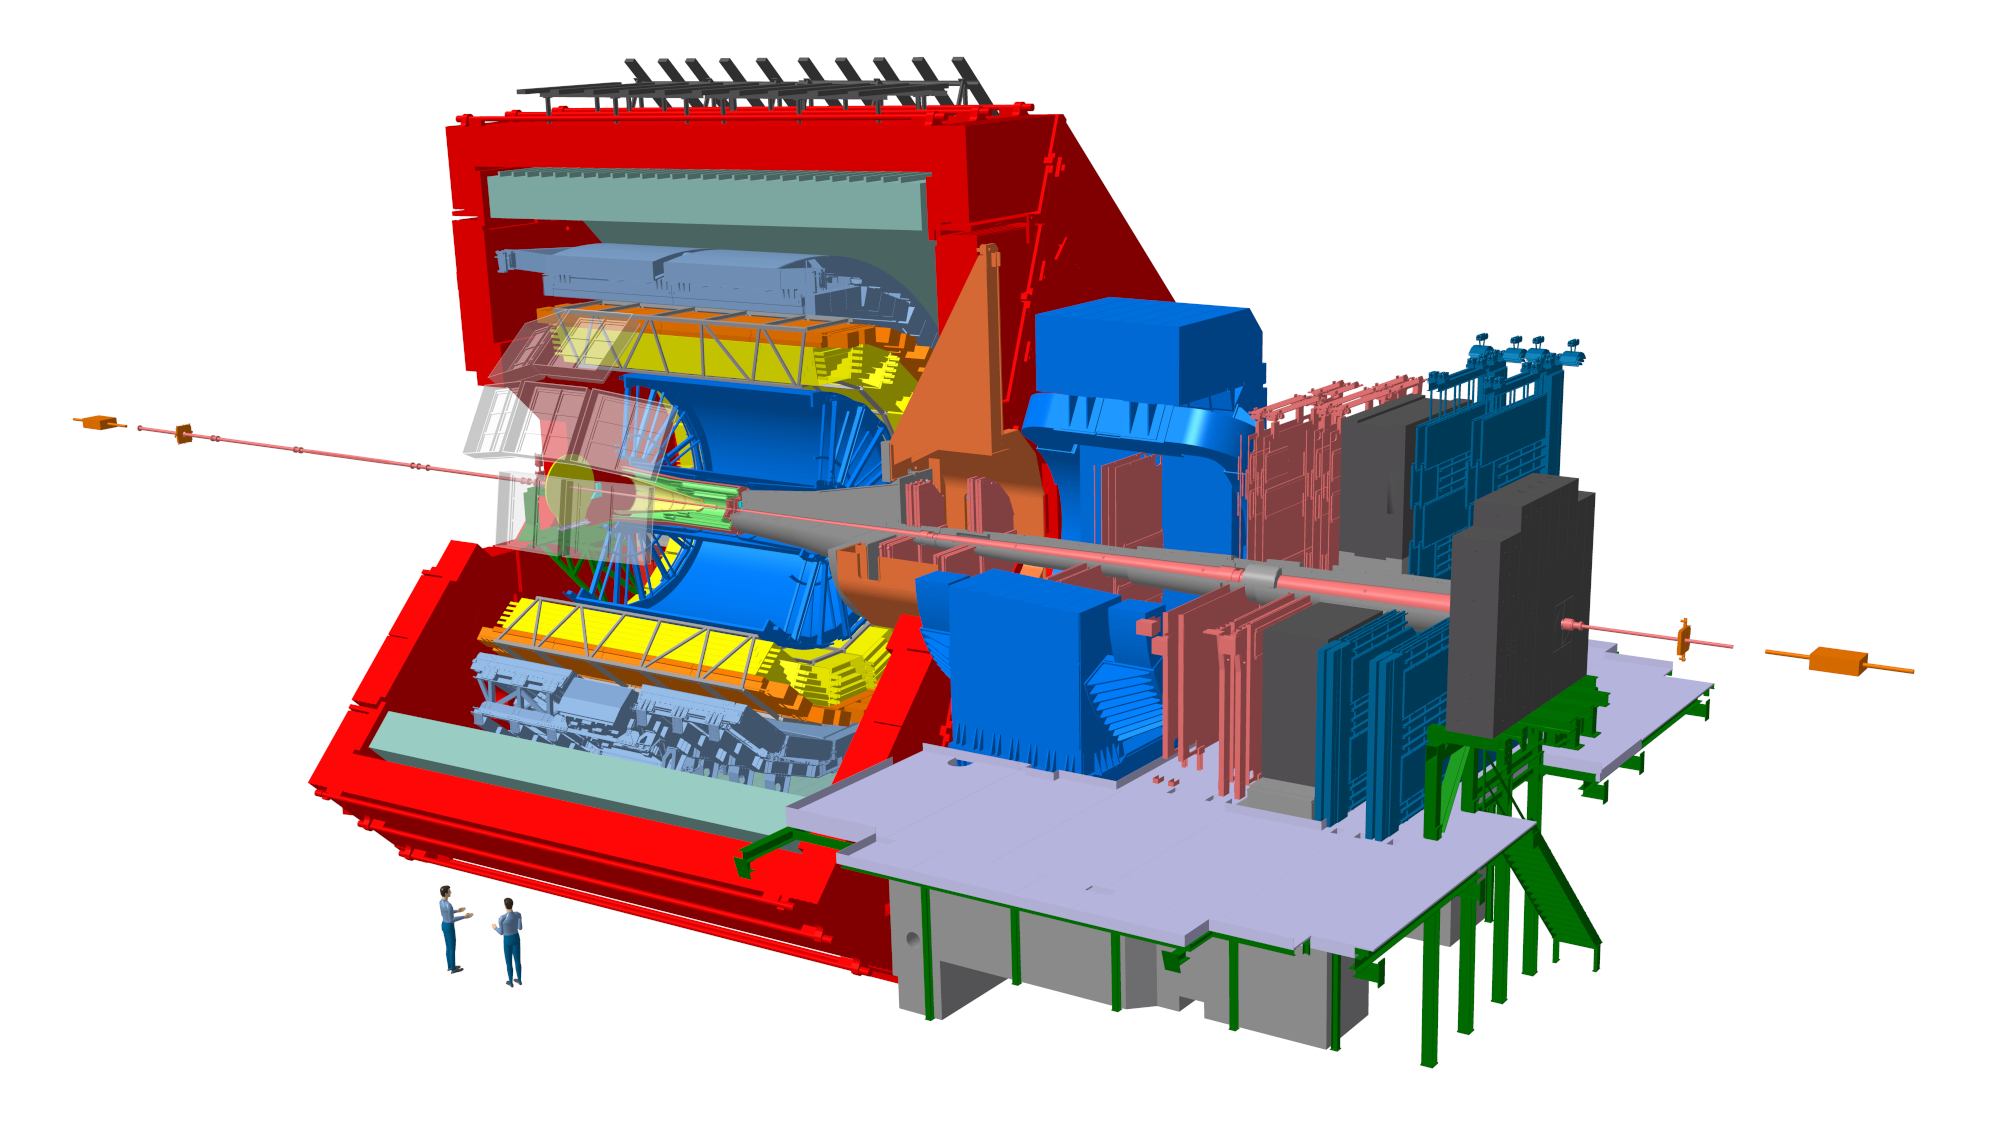
\includegraphics[width=0.8\textwidth]{Master/figs/alice_detectors.jpg}
    \caption[Figure text in list of figs]{Figure text in main text. (Remember citation)}
    \label{fig:alice-detector}
\end{figure}

\section{List}
\label{sec:list}

\begin{itemize}
    \item First
    \item Second
    \item Third
\end{itemize}

\section{Tables}
\label{sec:table}
% Use https://www.tablesgenerator.com/latex_tables#
% to generate tables, copy then into text

\begin{table}[ht]
    \centering
    \caption[Overview of clock domains]{Clock domain overview with frequencies and description.}
    \label{tab:clk-domains}
    \resizebox{\textwidth}{!}{%
    \begin{tabular}{@{}|l|r|l|@{}}
        \hline
        \rowcolor{tabledarkgray} 
                                            & \textbf{Clock Frequency} & \textbf{Description} \\ \hline
        \textbf{refclk\_i}                  & 320 \MHz{}               & \begin{tabular}[c]{@{}l@{}}Reference clock for the receivers \\ generated on the base-board\end{tabular}                    \\ \hline
        \rowcolor{tablelightgray} 
        \textbf{clk33\_i}                   & 33.3 \MHz{}              & \begin{tabular}[c]{@{}l@{}}Reference clock for the Clock Controller \\ generated by the system-on-chip\end{tabular}         \\ \hline
        \textbf{clk160\_i}                  & 160 \MHz{}               & \begin{tabular}[c]{@{}l@{}}Reference clock for the Clock Controller \\ generated on the base-board\end{tabular}             \\ \hline
        \rowcolor{tablelightgray}
        \textbf{system\_clk}                & 100 \MHz{}               & \begin{tabular}[c]{@{}l@{}}Main clock for the test system\end{tabular}                                                      \\ \hline
        \textbf{data\_clk}                  & 160 \MHz{}               & \begin{tabular}[c]{@{}l@{}}Clock used for the data path\end{tabular}                                                        \\ \hline
        \rowcolor{tablelightgray}
        \textbf{slow\_control\_fast\_clk}   & 80 \MHz{}                & \begin{tabular}[c]{@{}l@{}}Clock used for Slow Control modules\end{tabular}                                                 \\ \hline
        \textbf{lhc\_clk}                   & 40 \MHz{}                & \begin{tabular}[c]{@{}l@{}}Clock used for the sync generator \\ synchronized to the frequency of the \acs{lhc}\end{tabular} \\ \hline
        \rowcolor{tablelightgray}
        \textbf{testout\_oversampling\_clk} & 640 \MHz{}               & \begin{tabular}[c]{@{}l@{}}Clock used for the testout deserializer\end{tabular}                                            \\ \hline
    \end{tabular}%
    }
\end{table}

\section{Listings}
\label{sec:listings}

\begin{lstlisting}[
    language=Python, 
    caption={[Test bench driver definition]Test bench example: driver definition.}, 
    label=lst:tb-driver-def, 
    float=!htbp
    ]
def get_ipb(dut):
ipbus = IpBusDriver(
    dut,
    "ipbus",
    dut.ipb_clk,
    dut.ipb_in.ipb_addr,
    dut.ipb_in.ipb_wdata,
    dut.ipb_in.ipb_strobe,
    dut.ipb_in.ipb_write,
    dut.ipb_out.ipb_rdata,
    dut.ipb_out.ipb_ack,
    dut.ipb_out.ipb_err,
)
return ipbus
\end{lstlisting}

\section{Citation}
\label{sec:citation}

Citations referencing this statement come before punctuation \cite{safety}. 
Citations referencing the whole paragraph come at the very end of the paragraph, after punctuation. \cite{aluminium_LUT}

\section{Footnotes}
\label{sec:foot}

This is how you use a footnote\footnote{This is a footnote.}.